\documentclass[../../main.tex]{subfiles}

\graphicspath{{\subfix{../../immagini/}}}

\begin{document}
    Vengono ora presentati i risultati ottenuti inserendo le due categorie di classificatore all'interno dei filtri appresi. Come brevemente spiegato nel paragrafo \ref{sec:Esperimenti}, i risultati del precedente paragrafo possono essere utilizzati solamente per fornire un'idea dell'efficacia dei classificatori nel problema di riconoscimento degli URL. In questo secondo blocco di esperimenti, infatti, l'obiettivo è trovare il classificatore che porti alla maggiore diminuzione in termini di spazio dei filtri. Di fatto vogliamo quindi cercare un tradeoff tra prestazioni e spazio occupato.

    Il classificatore migliore in questo caso non può essere trovato tramite una classica model selection: nessuna metrica, infatti, risulta adatta a quantificare la bontà di un modello in termini di spazio occupato. Una model selection risulterebbe di conseguenza inadatta perché non avremmo nessuna metrica da massimizzare.

    Il numero di neuroni del percettrone viene quindi scelto in modo da ottenere un modello con una taglia molto vicina a quella della GRU a 16 dimensioni. Inoltre, dai risultati dello scorso paragrafo è possibile notare come, aumentando di molto il numero di neuroni, l'aumento delle prestazioni non sia altrettanto significativo. Per questo motivo viene testato un ulteriore modello con un numero inferiore di neuroni, scelto arbitrariamente, al fine di evidenziare eventuali miglioramenti nella dei taglia filtri appresi dovuti ad una dimensione minore del modello.

    Secondo questo ragionamento, viene testata una configurazione con 30 neuroni, che ha una grandezza molto simile alla GRU 16, e una configurazione con 20 neuroni. In entrambi casi il learning rate viene fissato a 0.001, dai risultati del precedente paragrafo sembra infatti la scelta migliore.
    
    \subsubsection{Scelta della soglia $\tau$}
    Una volta scelti a priori il tasso di falsi positivi desiderato $f$ e il tasso di falsi positivi del classificatore, in questo paragrafo chiamato $f_{\tau}$, la soglia $\tau$ ha un valore pari al quantile $100 \cdot (1 - f_{\tau})$ della distribuzione di probabilità, ritornata dal classificatore, delle non-chiavi presenti nell'insieme d'addestramento.

    Coerentemente con quanto detto nel paragrafo \ref{sec:falseProbLBF}, vengono testati diversi valori di $\tau$ variando il valore del rapporto $r_{\tau} = f_{\tau}/f$. Importante notare che, a seconda  del filtro considerato, dovranno valere le condizioni su $f_{\tau}$ descritte nel capitolo \ref{chap:filtriAppresi}.

    \subsubsection{Risultati filtro di Bloom}

    Vengono riportate in tabella \ref{tab:taglieFiltro} le taglie dei filtri di Bloom inizializzati sull'insieme delle chiavi $\mathcal{K}$, queste verranno utilizzate come base per confrontare le performance dei filtri appresi riportate successivamente.

    Una volta fissato $f$, le taglie sono state calcolate secondo l'equazione \ref{eqn:nlowerbound}.
    
    \begin{table}[H]
        \centering
        \begin{tabular}{lcccc}
            \toprule
            {} & \multicolumn{4}{c}{\textbf{FPR $f$}}\\
            {} & 0.001 & 0.005 & 0.01 & 0.02\\
            \midrule
            \textbf{Dimensione (KByte)} & 76.774 & 58.887 & 51.212 & 43.479\\
            \bottomrule
        \end{tabular}
        \caption{Taglie dei filtri di Bloom.}
        \label{tab:taglieFiltro}
    \end{table}

    \subsubsection{Risultati LBF}
    Le figure \ref{fig:percettroneEmpiricoLBF} e \ref{fig:GRUEmpiricoLBF} mostrano graficamente i risultati delle analisi empiriche, al variare del rapporto $r_{\tau}$, delle due tipologie di classificatore; la figure \ref{fig:tagliePercettroniLBF} e \ref{fig:taglieGRULBF}, invece, mostrano le taglie dell'intero LBF. In questo caso deve valere $0 < r_{\tau} < 1$, il rapporto viene quindi fatto variare tra questi due valori.

    Nello specifico, le figure \ref{fig:LBFFNRPercettrone20} e \ref{fig:LBFFNRPercettrone30} per il percettrone, e \ref{fig:LBFFNR_GRU16}, \ref{fig:LBFFNR_GRU8} e \ref{fig:LBFFNR_GRU4} per la GRU, mostrano il tasso di falsi negativi prodotti dal classificatore al variare del rapporto $r_{\tau}$. Si nota in tutte le figure una diminuzione del rapporto di falsi negativi all'aumentare di $r_{\tau}$, ciò è sensato: all'aumentare di $r_{\tau}$ il valore della soglia $\tau$ diminuisce, di conseguenza è più probabile che una chiave venga classificata come tale, generando un numero di falsi negativi via via minore.

    \begin{figure}[H]
        \centering
        \begin{subfigure}[b]{0.49\textwidth}
            \centering
            \includegraphics[width = \textwidth]{immagini/7/LBF/Percettrone(20, 0.001)_FNR.png}
            \caption{Rapporto dei falsi negativi prodotti dal percettrone (20, 0.001).}
            \label{fig:LBFFNRPercettrone20}
        \end{subfigure}
        \begin{subfigure}[b]{0.49\textwidth}
            \centering
            \includegraphics[width = \textwidth]{immagini/7/LBF/Percettrone(30, 0.001)_FNR.png}
            \caption{Rapporto dei falsi negativi prodotti dal percettrone (30, 0.001).}
            \label{fig:LBFFNRPercettrone30}
        \end{subfigure}
        \begin{subfigure}[b]{0.49\textwidth}
            \centering
            \includegraphics[width = \textwidth]{immagini/7/LBF/Percettrone(20, 0.001)_FPR.png}
            \caption{Tasso empirico di falsi positivi del percettrone (20, 0.001).}
            \label{fig:LBFFPRPercettrone20}
        \end{subfigure}
        \begin{subfigure}[b]{0.49\textwidth}
            \centering
            \includegraphics[width = \textwidth]{immagini/7/LBF/Percettrone(30, 0.001)_FPR.png}
            \caption{Tasso empirico di falsi positivi del percettrone (30, 0.001).}
            \label{fig:LBFFPRPercettrone30}
        \end{subfigure}
        \caption{Misurazioni empiriche sui percettroni.}
        \label{fig:percettroneEmpiricoLBF}
    \end{figure}

    \begin{figure}[H]
        \centering
        \begin{subfigure}[b]{0.32\textwidth}
            \centering
            \includegraphics[width = \textwidth]{immagini/7/LBF/GRU16_FNR.png}
            \caption{Rapporto dei falsi negativi prodotti dalla GRU 16.}
            \label{fig:LBFFNR_GRU16}
        \end{subfigure}
        \begin{subfigure}[b]{0.32\textwidth}
            \centering
            \includegraphics[width = \textwidth]{immagini/7/LBF/GRU8_FNR.png}
            \caption{Rapporto dei falsi negativi prodotti dalla GRU 8.}
            \label{fig:LBFFNR_GRU8}
        \end{subfigure}
        \begin{subfigure}[b]{0.32\textwidth}
            \centering
            \includegraphics[width = \textwidth]{immagini/7/LBF/GRU4_FNR.png}
            \caption{Rapporto dei falsi negativi prodotti dalla GRU 4.}
            \label{fig:LBFFNR_GRU4}
        \end{subfigure}
        \begin{subfigure}[b]{0.32\textwidth}
            \centering
            \includegraphics[width = \textwidth]{immagini/7/LBF/GRU16_FPR.png}
            \caption{Tasso empirico di falsi positivi della GRU 16.}
            \label{fig:LBFFPR_GRU16}
        \end{subfigure}
        \begin{subfigure}[b]{0.32\textwidth}
            \centering
            \includegraphics[width = \textwidth]{immagini/7/LBF/GRU8_FPR.png}
            \caption{Tasso empirico di falsi positivi della GRU 8.}
            \label{fig:LBFFPR_GRU8}
        \end{subfigure}
        \begin{subfigure}[b]{0.32\textwidth}
            \centering
            \includegraphics[width = \textwidth]{immagini/7/LBF/GRU4_FPR.png}
            \caption{Tasso empirico di falsi positivi della GRU 4.}
            \label{fig:LBFFPR_GRU4}
        \end{subfigure}
        \caption{Misurazioni empiriche sulle GRU.}
        \label{fig:GRUEmpiricoLBF}
    \end{figure}

    Le figure \ref{fig:LBFFPRPercettrone20}, \ref{fig:LBFFPRPercettrone30}, \ref{fig:LBFFPR_GRU16}, \ref{fig:LBFFPR_GRU8} e \ref{fig:LBFFPR_GRU4}, invece, mostrano il tasso di falsi positivi $f$ dell'intero LBF, calcolato sull'insieme di test composto di soli URL legittimi. In questo caso, come previsto, il tasso empirico rimane sempre stabile attorno al tasso atteso.

    Infine, le figure \ref{fig:LBFTagliaPercettrone20}, \ref{fig:LBFTagliaPercettrone30}, \ref{fig:LBFTagliaGRU16}, \ref{fig:LBFTagliaGRU8} e \ref{fig:LBFTagliaGRU4} mostrano le taglie dei rispettivi classificatori al variare di $r_{\tau}$. Confrontando i risultati di percettrone e GRU si nota come, in tutti i casi, le due configurazioni di percettrone occupino uno spazio inferiore rispetto alle GRU. Inoltre, è facile notare che i filtri appresi con GRU non siano quasi mai migliori rispetto ai corrispettivi filtri di Bloom, al contrario, i percettroni sembrano occupare uno spazio minore rispetto ai relativi filtri. 

    Confrontando invece le taglie occupate dalle due configurazioni di percettrone, si nota come il modello a 20 neuroni sembri leggermente migliore rispetto a quello a 30. Questo conferma quanto supposto inizialmente: seppur il modello a 30 neuroni sia migliore, in termini di performance, rispetto a quello a 20, quest'ultimo risulta migliore se inserito all'interno di un filtro appreso. Le performance guadagnate, non sono quindi sufficienti a giustificare l'aumento di spazio del modello.

    \begin{figure}[H]
        \centering
        \begin{subfigure}[b]{0.49\textwidth}
            \centering
            \includegraphics[width = \textwidth]{immagini/7/LBF/Percettrone(20, 0.001)_Taglia.png}
            \caption{Taglia del percettrone (20, 0.001)}
            \label{fig:LBFTagliaPercettrone20}
        \end{subfigure}
        \begin{subfigure}[b]{0.49\textwidth}
            \centering
            \includegraphics[width = \textwidth]{immagini/7/LBF/Percettrone(30, 0.001)_Taglia.png}
            \caption{Taglia del percettrone (30, 0.001)}
            \label{fig:LBFTagliaPercettrone30}
        \end{subfigure}
        \caption{Taglie dei percettroni.}
        \label{fig:tagliePercettroniLBF}
    \end{figure}

    \begin{figure}[H]
        \centering
        \begin{subfigure}[b]{0.32\textwidth}
            \centering
            \includegraphics[width = \textwidth]{immagini/7/LBF/GRU16_Taglia.png}
            \caption{Taglia della GRU 16.}
            \label{fig:LBFTagliaGRU16}
        \end{subfigure}
        \begin{subfigure}[b]{0.32\textwidth}
            \centering
            \includegraphics[width = \textwidth]{immagini/7/LBF/GRU8_Taglia.png}
            \caption{Taglia della GRU 8.}
            \label{fig:LBFTagliaGRU8}
        \end{subfigure}
        \begin{subfigure}[b]{0.32\textwidth}
            \centering
            \includegraphics[width = \textwidth]{immagini/7/LBF/GRU4_Taglia.png}
            \caption{Taglia della GRU 4.}
            \label{fig:LBFTagliaGRU4}
        \end{subfigure}
        \caption{Taglie delle GRU.}
        \label{fig:taglieGRULBF}
    \end{figure}

    \subsubsection{Risultati SLBF}
    Anche in questo caso nelle figure \ref{fig:percettroneEmpiricoSLBF} e \ref{fig:GRUEmpiricoSLBF} vengono presentati i risultati empirici sulle strutture, nelle figure \ref{fig:tagliePercettroniSLBF} e \ref{fig:taglieGRUSLBF}, invece, le rispettive taglie. In questo caso la condizione su $r_{\tau}$ è $(1 - m_b/m) \leq r_{\tau} \leq 1/f \cdot \left(1 - m_b/m\right)$.
    \begin{figure}[H]
        \centering
        \begin{subfigure}[b]{0.49\textwidth}
            \centering
            \includegraphics[width = \textwidth]{immagini/7/SLBF/Percettrone(20, 0.001)_FNR.png}
            \caption{Rapporto dei falsi negativi prodotti dal Percettrone (20, 0.001).}
            \label{fig:SLBFFNRPercettrone20}
        \end{subfigure}
        \begin{subfigure}[b]{0.49\textwidth}
            \centering
            \includegraphics[width = \textwidth]{immagini/7/SLBF/Percettrone(30, 0.001)_FNR.png}
            \caption{Rapporto dei falsi negativi prodotti dal Percettrone (30, 0.001).}
            \label{fig:SLBFFNRPercettrone30}
        \end{subfigure}
        \begin{subfigure}[b]{0.49\textwidth}
            \centering
            \includegraphics[width = \textwidth]{immagini/7/SLBF/Percettrone(20, 0.001)_FPR.png}
            \caption{Tasso empirico di falsi positivi del Percettrone (20, 0.001).}
            \label{fig:SLBFFPRPercettrone20}
        \end{subfigure}
        \begin{subfigure}[b]{0.49\textwidth}
            \centering
            \includegraphics[width = \textwidth]{immagini/7/SLBF/Percettrone(30, 0.001)_FPR.png}
            \caption{Tasso empirico di falsi positivi del Percettrone (30, 0.001).}
            \label{fig:SLBFFPRPercettrone30}
        \end{subfigure}
        \caption{Misurazioni empiriche sui percettroni.}
        \label{fig:percettroneEmpiricoSLBF}
    \end{figure}

    \begin{figure}[H]
        \centering
        \begin{subfigure}[b]{0.32\textwidth}
            \centering
            \includegraphics[width = \textwidth]{immagini/7/SLBF/GRU16_FNR.png}
            \caption{Rapporto dei falsi negativi prodotti dalla GRU 16.}
            \label{fig:SLBFFNR_GRU16}
        \end{subfigure}
        \begin{subfigure}[b]{0.32\textwidth}
            \centering
            \includegraphics[width = \textwidth]{immagini/7/SLBF/GRU8_FNR.png}
            \caption{Rapporto dei falsi negativi prodotti dalla GRU 8.}
            \label{fig:SLBFFNR_GRU8}
        \end{subfigure}
        \begin{subfigure}[b]{0.32\textwidth}
            \centering
            \includegraphics[width = \textwidth]{immagini/7/SLBF/GRU4_FNR.png}
            \caption{Rapporto dei falsi negativi prodotti dalla GRU 4.}
            \label{fig:SLBFFNR_GRU4}
        \end{subfigure}
        \begin{subfigure}[b]{0.32\textwidth}
            \centering
            \includegraphics[width = \textwidth]{immagini/7/SLBF/GRU16_FPR.png}
            \caption{Tasso empirico di falsi positivi della GRU 16.}
            \label{fig:SLBFFPR_GRU16}
        \end{subfigure}
        \begin{subfigure}[b]{0.32\textwidth}
            \centering
            \includegraphics[width = \textwidth]{immagini/7/SLBF/GRU8_FPR.png}
            \caption{Tasso empirico di falsi positivi della GRU 8.}
            \label{fig:SLBFFPR_GRU8}
        \end{subfigure}
        \begin{subfigure}[b]{0.32\textwidth}
            \centering
            \includegraphics[width = \textwidth]{immagini/7/SLBF/GRU4_FPR.png}
            \caption{Tasso empirico di falsi positivi della GRU 4.}
            \label{fig:SLBFFPR_GRU4}
        \end{subfigure}
        \caption{Misurazioni empiriche sulle GRU.}
        \label{fig:GRUEmpiricoSLBF}
    \end{figure}

    Il ragionamento già fatto per gli LBF può essere ripetuto anche in questo caso: il tasso di falsi negativi del classificatore diminuisce all'aumentare di $r_{\tau}$, e il tasso di falsi positivi empirico è sempre molto vicino a quello atteso.

    Nelle figure \ref{fig:SLBFFNRPercettrone20}, \ref{fig:SLBFFNRPercettrone30}, \ref{fig:SLBFFNR_GRU16}, \ref{fig:SLBFFNR_GRU8} e \ref{fig:SLBFFNR_GRU4} si nota però una differenza rispetto ai risultati precedenti: il tasso di falsi negativi decresce molto più rapidamente rispetto a ciò che accade nei rispettivi LBF, in alcuni casi arrivando quasi a zero. Questo accade a causa di valori di $f_\tau$ testati più alti, che portano a valori di $\tau$ più bassi.

    Il tasso di falsi negativi molto basso è utile a spiegare l'andamento dei grafici \ref{fig:SLBFTagliaPercettrone20}, \ref{fig:SLBFTagliaPercettrone30}, \ref{fig:SLBFTagliaGRU16}, \ref{fig:SLBFTagliaGRU8} e \ref{fig:SLBFTagliaGRU4}, che mostrano le taglie delle strutture al variare di $r_\tau$. Nella figura \ref{fig:SLBFTagliaPercettrone20}, ad esempio, l'andamento della curva $f = 0.02$ è crescente, ciò è giustificabile ricordando come vengono calcolate le taglie $n_{b0}$ e $n_b$ (equazione \ref{eqn:SLBFGrandezzaOttimaInit} e \ref{eqn:SLBFGrandezzaOttima}). Se il numero di falsi negativi $m_b$ tende a 0 allora la grandezza del filtro di backup $n_b$ tenderà anch'essa a 0, viceversa, la taglia del filtro $n_{b0}$ continuerà a crescere, generando l'andamento crescente evidenziato dalla figura.

    Anche in questo caso, confrontando le figure \ref{fig:tagliePercettroniSLBF} \ref{fig:taglieGRUSLBF}, sembra che il percettrone risulti migliore per ogni $f$ testato. Interessante notare come, però, in questo caso anche la GRU fornisca prestazioni migliori in termini di spazio rispetto al filtro base.

    \begin{figure}[H]
        \centering
        \begin{subfigure}[b]{0.49\textwidth}
            \centering
            \includegraphics[width = \textwidth]{immagini/7/SLBF/Percettrone(20, 0.001)_Taglia.png}
            \caption{Taglia del percettrone (20, 0.001)}
            \label{fig:SLBFTagliaPercettrone20}
        \end{subfigure}
        \begin{subfigure}[b]{0.49\textwidth}
            \centering
            \includegraphics[width = \textwidth]{immagini/7/SLBF/Percettrone(30, 0.001)_Taglia.png}
            \caption{Taglia del percettrone (30, 0.001)}
            \label{fig:SLBFTagliaPercettrone30}
        \end{subfigure}
        \caption{Taglie dei percettroni.}
        \label{fig:tagliePercettroniSLBF}
    \end{figure}

    \begin{figure}[H]
        \centering
        \begin{subfigure}[b]{0.32\textwidth}
            \centering
            \includegraphics[width = \textwidth]{immagini/7/SLBF/GRU16_Taglia.png}
            \caption{Taglia della GRU 16.}
            \label{fig:SLBFTagliaGRU16}
        \end{subfigure}
        \begin{subfigure}[b]{0.32\textwidth}
            \centering
            \includegraphics[width = \textwidth]{immagini/7/SLBF/GRU8_Taglia.png}
            \caption{Taglia della GRU 8.}
            \label{fig:SLBFTagliaGRU8}
        \end{subfigure}
        \begin{subfigure}[b]{0.32\textwidth}
            \centering
            \includegraphics[width = \textwidth]{immagini/7/SLBF/GRU4_Taglia.png}
            \caption{Taglia della GRU 4.}
            \label{fig:SLBFTagliaGRU4}
        \end{subfigure}
        \caption{Taglie delle GRU.}
        \label{fig:taglieGRUSLBF}
    \end{figure}

    \subsubsection{Confronto con codifica binaria}
    Vengono ora presentati i risultati ottenuti utilizzando la codifica binaria presentata nel paragrafo \ref{sec:implementazione}. Da alcuni esperimenti è emerso che addestrare il percettrone utilizzando questa codifica porti, a parità di iperparametri, a delle performance migliori. 
    
    Il problema principale è che utilizzando questa tipologia di codifica la dimensione dei vettori in ingresso aumenta notevolmente, aumentando di conseguenza la taglia del modello. Nel nostro dataset, ad esempio, la codifica con count vectorizer porta a vettori di dimensione 82, mentre usando questa codifica (troncando a 30 caratteri), i vettori hanno dimensione 210. Per ovviare a questo problema la soluzione è ridurre il numero di neuroni nascosti, riducendo di conseguenza il numero totale di parametri del modello.

    Le figure \ref{fig:tagliePercettroniBinLBF} e \ref{fig:tagliePercettroniBinSLBF} mostrano le taglie dei filtri ottenuti utilizzando la codifica binaria e 8 neuroni per lo strato nascosto (con un numero totale di parametri vicino a quello della rete a 20 neuroni).

    \begin{figure}[H]
        \centering
        \begin{subfigure}[b]{0.48\textwidth}
            \centering
            \includegraphics[width=\textwidth]{immagini/7/LBF/Percettrone(8, 0.001) Binario_Taglia.png}
            \caption{}
        \end{subfigure}
        \begin{subfigure}[b]{0.48\textwidth}
            \centering
            \includegraphics[width=\textwidth]{immagini/7/LBF/Percettrone(20, 0.001)_Taglia.png}
            \caption{}
        \end{subfigure}
        \caption{Taglie dei percettroni (LBF).}
        \label{fig:tagliePercettroniBinLBF}
    \end{figure}

    \begin{figure}[H]
        \centering
        \begin{subfigure}[b]{0.48\textwidth}
            \centering
            \includegraphics[width=\textwidth]{immagini/7/SLBF/Percettrone(8, 0.001) Binario_Taglia.png}
            \caption{}
        \end{subfigure}
        \begin{subfigure}[b]{0.48\textwidth}
            \centering
            \includegraphics[width=\textwidth]{immagini/7/SLBF/Percettrone(20, 0.001)_Taglia.png}
            \caption{}  
        \end{subfigure}
        \caption{Taglie dei percettroni (SLBF).}
        \label{fig:tagliePercettroniBinSLBF}
    \end{figure}

    Seppur il percettrone binario abbia performance migliori rispetto alle GRU presentate, il percettrone con la codifica utilizzata fino ad ora risulta comunque migliore. Per questo motivo verranno riportati di seguito solamente i risultati relativi alla prima codifica.


    \subsubsection{Confronto tra filtri di Bloom, LBF e SLBF}
    Le tabelle \ref{tab:confrontoFinaleLBF} e \ref{tab:confrontoFinaleSLBF} mettono a confronto le taglie degli LBF generati da ognuno dei classificatori nel caso migliore. In entrambe le tipologie di filtro il percettrone a 20 neuroni risulta essere la scelta migliore. Inoltre, per ogni $f$ testato, l'SLBF fornisce un miglioramento più ampio rispetto al relativo LBF.

    \begin{table}[H]
        \centering
        \begin{tabular}{llcccc}
            \toprule
            {} & {}  & \multicolumn{4}{c}{\textbf{FPR $f$}}\\
            {} & {}  & 0.001 & 0.005 & 0.01 & 0.02\\
            \midrule
            \multicolumn{6}{c}{\textbf{Filtro di Bloom}}\\
            \midrule
            {} & $n$ & 76.774 & 58.887 & 51.212 & 43.479\\
            \midrule 
            \multicolumn{6}{c}{\textbf{LBF}}\\
            \midrule
            \multirow{2}{*}{\textbf{Perc. (20, 0.001)}} & $n$ &  \cellcolor{red!25}67.881 & \cellcolor{red!25}40.821 & \cellcolor{red!25}29.649 & \cellcolor{red!25}20.554\\
            & $n_c$ & 6.809 &  6.809 &  6.809 &  6.809 \\
            \hdashline 
            \multirow{2}{*}{\textbf{Perc. (30, 0.001)}} & $n$ & 68.420 & 41.536 & 30.983 & 22.581\\
            & $n_c$ & 10.090 & 10.090 & 10.090 & 10.090\\   
            \hdashline 
            \multirow{2}{*}{\textbf{GRU 16}} & $n$ & 85.676 & 66.307 & 52.265 & 35.646\\
            & $n_c$ & 9.671 &  9.671 &  9.671 &  9.671\\
            \hdashline 
            \multirow{2}{*}{\textbf{GRU 8}}& $n$ & 79.955 & 60.030 & 49.810 & 40.047\\
            & $n_c$&  6.701 &  6.701 &  6.701 &  6.701\\
            \hdashline 
            \multirow{2}{*}{\textbf{GRU 4}}& $n$ & 80.557 & 62.734 & 54.656 & 45.309\\
            & $n_c$ &  5.779 &  5.779 &  5.779 &  5.779\\ 
            \bottomrule
        \end{tabular}
        \caption{Confronto della taglia degli LBF nel caso del rapporto $r_{\tau}$ migliore. Vengono evidenziate le celle corrispondenti alla taglia più bassa. Tutte le taglie riportate sono in KByte. La notazione $n_c$ indica la taglia del classificatore.}
        \label{tab:confrontoFinaleLBF}
    \end{table}

    \begin{table}[H]
        \centering
        \begin{tabular}{llcccc}
            \toprule
            {} & {}  & \multicolumn{4}{c}{\textbf{FPR $f$}}\\
            {} & {}  & 0.001 & 0.005 & 0.01 & 0.02\\
            \midrule
            \multicolumn{6}{c}{\textbf{Filtro di Bloom}}\\
            \midrule
            {} & $n$ & 76.774 & 58.887 & 51.212 & 43.479\\
            \midrule 
            \multicolumn{6}{c}{\textbf{SLBF}}\\
            \midrule           
            \multirow{4}{*}{\textbf{Perc. (20, 0.001)}} & $n$ & \cellcolor{red!25}54.585  & \cellcolor{red!25}35.823 & \cellcolor{red!25}28.119 & \cellcolor{red!25}20.415\\
            & $n_{b0}$ & 29.575 & 17.746 & 10.042 &  2.338\\
            & $n_{b}$ & 18.201 & 11.268 & 11.268 & 11.268\\
            & $n_c$ &  6.809 &  6.809 &  6.809 &  6.809\\
            \hdashline 
            \multirow{4}{*}{\textbf{Perc. (30, 0.001)}} & $n$ & 55.981 & 37.953 & 30.325 & 22.622\\
            & $n_{b0}$ & 29.096 & 14.870 &  9.799 &  2.095\\
            & $n_{b}$ & 16.795 & 12.993 & 10.436 & 10.436\\
            & $n_c$ & 10.090 & 10.090 & 10.090 & 10.090\\
            \hdashline 
            \multirow{4}{*}{\textbf{GRU 16}} & $n$   & 71.822 & 46.744 & 39.086 & 31.411\\
            & $n_{b0}$ & 34.894 & 26.986 & 20.203 & 10.584\\
            & $n_{b}$ & 27.258 & 10.087 &  9.212 & 11.155\\
            & $n_c$ &  9.671 &  9.671 &  9.671 &  9.671\\
            \hdashline 
            \multirow{4}{*}{\textbf{GRU 8}} & $n$  & 72.834 & 44.386 & 36.040 & 28.443\\
            & $n_{b0}$ & 37.367 & 28.068 & 23.094 & 14.082\\
            & $n_{b}$ & 28.765 &  9.617 &  6.245 &  7.660\\
            & $n_c$ &  6.701 &  6.701 &  6.701 &  6.701\\
            \hdashline 
            \multirow{4}{*}{\textbf{GRU 4}} & $n$  & 77.271 & 52.095 & 40.479 & 30.176\\
            & $n_{b0}$ & 42.709 & 31.346 & 27.628 & 22.101\\
            & $n_{b}$ & 28.782 & 14.970 &  7.073 &  2.296\\
            & $n_c$ &  5.779 &  5.779 &  5.779 &  5.779\\
            \bottomrule          
        \end{tabular}
        \caption{Confronto della taglia degli SLBF nel caso del rapporto $r_{\tau}$ migliore. Vengono evidenziate le celle corrispondenti alla taglia più bassa. Tutte le taglie riportate sono in KByte. La notazione $n_c$ indica la taglia del classificatore.}
        \label{tab:confrontoFinaleSLBF}
    \end{table}

    \subsubsection{Tempi di accesso}
    Un ultimo aspetto importante da considerare è il tempo di accesso ad ognuno delle tipologie di filtro proposte. Le tabelle \ref{tab:tempiMediLBF} e \ref{tab:tempiMediSLBF} mostrano i tempi medi d'accesso per elemento, rispettivamente per LBF ed SLBF. I tempi per elemento vengono calcolati misurando il tempo di accesso sull'insieme di testing, e dividendo questo tempo per la cardinalità del testing set.

    Dalle tabelle emerge che il filtro di Bloom classico risulta più veloce di circa 1-2 ordini di grandezza, a seconda del classificatore considerato, rispetto alle controparti apprese. La minore efficienza in termini di tempo dei filtri appresi è molto probabilmente dovuta alla maggiore complessità della struttura: nel filtro di Bloom, infatti, l'accesso consiste semplicemente nel calcolo delle funzioni di hash, mentre nelle strutture apprese è necessario anche interrogare il classificatore per ottenere i valori delle predizioni; più un classificatore è complesso, maggiore sarà il tempo necessario per questa operazione. Questo viene anche confermato dal fatto che i filtri che utilizzano la GRU 16 sono quelli con il tempo medio di acceso più alto.

    \begin{table}[H]
        \centering
        \begin{tabular}{lrrrr}
            \toprule
            & \multicolumn{4}{c}{\textbf{FPR} $f$}\\
            & 0.001 & 0.005 & 0.10 & 0.20\\        
            \midrule
            \textbf{Filtro di Bloom} & 9.976E-07 & 1.06E-06 & 9.41E-07 & 7.94E-07\\
            \midrule
            \textbf{Perc.} (20, 0.001) & 8.843E-06 & 8.814E-06 &  8.774E-06 & 8.770E-06\\
            \textbf{Perc.} (30, 0.001) & 8.848E-06 & 8.869E-06 &  8.826E-06 & 8.764E-06\\
            \textbf{GRU} 16 & 4.546E-05 & 4.545E-05 &  4.540E-05 & 4.542E-05\\
            \textbf{GRU} 8 &  2.180E-05 & 2.173E-05 &  2.174E-05 & 2.171E-05\\
            \textbf{GRU} 4 & 1.519E-05 & 1.516E-05 & 1.513E-05 & 1.511E-05\\
            \bottomrule
        \end{tabular}
        \caption{Tempi di accesso medi per elemento su LBF(calcolati su 5 iterazioni).}
        \label{tab:tempiMediLBF}
    \end{table}

    \begin{table}[H]
        \centering
        \begin{tabular}{lrrrr}
            \toprule
            & \multicolumn{4}{c}{\textbf{FPR} $f$}\\
            & 0.001 & 0.005 & 0.10 & 0.20\\        
            \midrule
            \textbf{Filtro di Bloom} & 9.976E-07 & 1.06E-06 & 9.41E-07 & 7.94E-07\\
            \midrule
            \textbf{Perc.} (20, 0.001) & 8.085E-06 & 8.189E-06 &  8.258E-06 & 8.203E-06\\
            \textbf{Perc.} (30, 0.001) & 8.135E-06 & 8.171E-06 &  8.231E-06 & 8.127E-06\\
            \textbf{GRU} 16 & 4.542E-05 & 4.552E-05 &  4.555E-05 & 4.555E-05\\
            \textbf{GRU} 8 &  1.972E-05 & 1.981E-05 &  1.985E-05 & 1.987E-05\\
            \textbf{GRU} 4 & 1.454E-05 & 1.464E-05 & 1.471E-05 & 1.471E-05\\
            \bottomrule
        \end{tabular}
        \caption{Tempi di accesso medi per elemento su SLBF(calcolati su 5 iterazioni).}
        \label{tab:tempiMediSLBF}
    \end{table}

    In ultimo, è interessante notare che i tempi dei SLBF siano simili e, in alcuni casi, leggermente migliori rispetto a quelli dei relativi LBF. Dato che l'SLBF comprende un filtro iniziale il numero di chiamate al classificatore è minore rispetto a un LBF, questo potrebbe giustificare i tempi più bassi della struttura a sandwich.
\end{document}